%%%%%%%%%%%%%%%%%%%%%%%%%%%%%%%%%%%%%%%%%%%%%%%%%%%%%%%%%%%%%%%%%%%%%%%%%%%%%%%%%%%%%%%%%%%%%%%%%%%
%
% Primordial Machine's Least Greatest Functors Library
% Copyright (C) 2017-2019 Michael Heilmann
%
% This software is provided 'as-is', without any express or implied warranty.
% In no event will the authors be held liable for any damages arising from the
% use of this software.
%
% Permission is granted to anyone to use this software for any purpose,
% including commercial applications, and to alter it and redistribute it
% freely, subject to the following restrictions:
%
% 1. The origin of this software must not be misrepresented;
%    you must not claim that you wrote the original software.
%    If you use this software in a product, an acknowledgment
%    in the product documentation would be appreciated but is not required.
%
% 2. Altered source versions must be plainly marked as such,
%    and must not be misrepresented as being the original software.
%
% 3. This notice may not be removed or altered from any source distribution.
%
%%%%%%%%%%%%%%%%%%%%%%%%%%%%%%%%%%%%%%%%%%%%%%%%%%%%%%%%%%%%%%%%%%%%%%%%%%%%%%%%%%%%%%%%%%%%%%%%%%%

\documentclass[oneside]{book}

%%%%%%%%%%%%%%%%%%%%%%%%%%%%%%%%%%%%%%%%%%%%%%%%%%%%%%%%%%%%%%%%%%%%%%%%%%%%%%%%%%%%%%%%%%%%%%%%%%%
%
% Primordial Machine Least Greatest Functors Library
% Copyright (c) 2017-2019 Michael Heilmann <michaelheilmann@primordialmachine.com>
%
% This software is provided 'as-is', without any express or implied warranty.
% In no event will the authors be held liable for any damages arising from the
% use of this software.
%
% Permission is granted to anyone to use this software for any purpose,
% including commercial applications, and to alter it and redistribute it
% freely, subject to the following restrictions:
%
% 1. The origin of this software must not be misrepresented;
%    you must not claim that you wrote the original software.
%    If you use this software in a product, an acknowledgment
%    in the product documentation would be appreciated but is not required.
%
% 2. Altered source versions must be plainly marked as such,
%    and must not be misrepresented as being the original software.
%
% 3. This notice may not be removed or altered from any source distribution.
%
%%%%%%%%%%%%%%%%%%%%%%%%%%%%%%%%%%%%%%%%%%%%%%%%%%%%%%%%%%%%%%%%%%%%%%%%%%%%%%%%%%%%%%%%%%%%%%%%%%%

\usepackage[utf8]{inputenc}
%
\usepackage{xparse}
\setcounter{tocdepth}{4} % Include subsubsections into ToC.
\setcounter{secnumdepth}{4} % Number subsubsection.
%
\usepackage{textcomp} % for \textlangle and \textrangle macros
\usepackage{xcolor}
%
\usepackage{xifthen}
%
\usepackage{datetime}
%
\usepackage{tabularx} % for tabularx environment
\usepackage{multirow}
%
\usepackage{lmodern}
\usepackage{microtype}
%
\usepackage{graphicx}
\usepackage[colorlinks]{hyperref}
\usepackage[margin=0.75in]{geometry}
\usepackage{amsmath,amssymb,amsfonts}

\setlength{\parindent}{0pt} % Disable paragraph indention.

\makeatletter

% "(Get|Set)Author".
% The name of the author.
\def\SetAuthor#1{\gdef\@author{#1}}
\def\@author{\@latex@warning@no@line{No author given}}
\def\GetAuthor{\@author}

% "(Get|Set)Email".
% The email (address) of the author.
\def\SetEmail#1{\gdef\@email{#1}}
\def\@email{\@latex@warning@no@line{No email given}}
\def\GetEmail{\@email}

% "(Get|Set)Organization".
% The organization the library is published by.
\def\SetOrganization#1{\gdef\@organization{#1}}
\def\@organization{\@latex@warning@no@line{No organization given}}
\def\GetOrganization{\@organization}

% "(Get|Set)LibraryName".
% The name of the library.
\def\SetLibraryName#1{\gdef\@libraryName{#1}}
\def\@libraryName{\@latex@warning@no@line{No library name given}}
\def\GetLibraryName{\@libraryName}

% "(Get|Set)LibraryIncludesPath".
% The includes directory path.
% Example: "primordialmachine/arithmetic-functors/$(PlatformTarget.toLower())/$(Configuration.toLower())/includes"
\def\SetLibraryIncludesDirectoryPath#1{\gdef\@libraryIncludesDirectoryPath{#1}}
\def\@libraryIncludesDirectoryPath{\@latex@warning@no@line{No library includes directory path given}}
\def\GetLibraryIncludesDirectoryPath{\@libraryIncludesDirectoryPath}

% "(Get|Set)LibraryIncludeFile".
% The include file name of the library.
% Example: "include.hpp".
\def\SetLibraryIncludeFileName#1{\gdef\@libraryIncludeFileName{#1}}
\def\@libraryIncludeFileName{\@latex@warning@no@line{No library include file name given}}
\def\GetLibraryIncludeFileName{\@libraryIncludeFileName}

% "(Get|Set)LibraryIncludeDirectiveFilePath".
% The library include directive file path.
% Example: "primordialmachine/arithmetic_functors/include.hpp".
\def\SetLibraryIncludeDirectiveFilePath#1{\gdef\@libraryIncludeDirectiveFilePath{#1}}
\def\@libraryIncludeDirectiveFilePath{\@latex@warning@no@line{No library include directive file path}}
\def\GetLibraryIncludeDirectiveFilePath{\@libraryIncludeDirectiveFilePath}

% "(Get|Set)LibraryStaticLibrariesDirectoryPath".
% The static libraries directory path.
% Example: "primordialmachine/arithmetic-functors/$(PlatformTarget.toLower())/$(Configuration.toLower())/libraries".
\def\SetLibraryStaticLibrariesDirectoryPath#1{\gdef\@libraryStaticLibrariesDirectoryPath{#1}}
\def\@libraryStaticLibrariesDirectoryPath{\@latex@warning@no@line{No library static libraries directory path given}}
\def\GetLibraryStaticLibrariesDirectoryPath{\@libraryStaticLibrariesDirectoryPath}

% "(Get|Set)LibraryStaticLibraryFileName.
% The static library file name of the library.
% Example: "arithmetic-functors.hpp".
\def\SetLibraryStaticLibraryFileName#1{\gdef\@libraryStaticLibraryFileName{#1}}
\def\@libraryStaticLibraryFileName{\@latex@warning@no@line{No library static library file name given}}
\def\GetLibraryStaticLibraryFileName{\@libraryStaticLibraryFileName}

% "(Get|Set)LibraryVersion".
% The version of the library.
\def\SetLibraryVersion#1{\gdef\@libraryVersion{#1}}
\def\@libraryVersion{\@latex@warning@no@line{No library version given}}
\def\GetLibraryVersion{\@libraryVersion}

% "(Get|Set)LibraryRepository".
% The repository (url) of the library.
\def\SetLibraryRepository#1{\gdef\@libraryRepository{#1}}
\def\@libraryRepository{\@latex@warning@no@line{No library repository given}}
\def\GetLibraryRepository{\@libraryRepository}

% "(Get|Set)DocumentType".
% The document type of this document.
\def\SetDocumentType#1{\gdef\@documentType{#1}}
\def\@documentType{\@latex@warning@no@line{No document type given}}
\def\GetDocumentType{\@documentType}

\let\tableofcontentsORIG\tableofcontents
\renewcommand\tableofcontents{\tableofcontentsORIG}

% Define "maketitle".
\def\maketitle{%
  \thispagestyle{empty}
  \begin{centering}

  \vspace*{6.0\baselineskip} % White space at the top of the page

  %%%%%%%%%%%%%%%%%%%%%%%%%%%%%%%%
  % TITLE
  %%%%%%%%%%%%%%%%%%%%%%%%%%%%%%%%

  \rule{\textwidth}{1.6pt}\vspace*{-\baselineskip}\vspace*{2pt} % Thick horizontal rule
  \rule{\textwidth}{0.4pt} % Thin horizontal rule

  \vspace{0.75\baselineskip} % Whitespace above the title

  {\normalsize\uppercase{\GetOrganization{}}'s}\\
  \vspace{1\baselineskip} % For some reason the lines are overlapping.
  {\LARGE\uppercase{\GetLibraryName} \uppercase{\GetLibraryVersion}}

  \vspace{0.75\baselineskip} % Whitespace below the title

  \rule{\textwidth}{0.4pt}\vspace*{-\baselineskip}\vspace{3.2pt} % Thin horizontal rule
  \rule{\textwidth}{1.6pt} % Thick horizontal rule

  \vspace{2\baselineskip} % Whitespace after the title block

  %%%%%%%%%%%%%%%%%%%%%%%%%%%%%%%%%
  % SUBTITLE
  %%%%%%%%%%%%%%%%%%%%%%%%%%%%%%%%%

  \vspace{2\baselineskip} % Whitespace after the title block

  \GetDocumentType % Subtitle or further description

  \vspace*{3\baselineskip} % Whitespace under the subtitle

  %%%%%%%%%%%%%%%%%%%%%%%%%%%%%%%%%
  % EDITORS
  %%%%%%%%%%%%%%%%%%%%%%%%%%%%%%%%%

  \vspace*{1\baselineskip} % Whitespace before editors

  Edited By

  \vspace{0.5\baselineskip} % Whitespace before the editors

  {\scshape\Large \GetAuthor \\
  {\normalsize(\href{mailto:\GetEmail}{\GetEmail})} \\} % Editor list

  \end{centering}

  %%%%%%%%%%%%%%%%%%%%%%%%%%%%%%%%%%
  % Footer
  %%%%%%%%%%%%%%%%%%%%%%%%%%%%%%%%%%
  \vspace*{\fill} % Whitespace before the editors
  \begin{tabularx}{\columnwidth}{m{0.75cm}m{4.75cm}X}
  \multirow{2}{=}{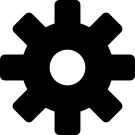
\includegraphics[scale=0.05]{primordialmachine-135x135.png}} & Primordial Machine                                                  & \hfill Created with \LaTeX\\
                                                                               & \href{https://primordialmachine.com}{https://primordialmachine.com} & \hfill Compiled on \today\ at \currenttime
  \end{tabularx}
}

\makeatother

\SetOrganization{Primordial Machine}
\SetLibraryName{Least Greatest Functors}
\SetLibraryVersion{0.1}
\SetLibraryRepository{https://github.com/primordialmachine/least-greatest-functors}
\SetAuthor{Michael Heilmann}
\SetEmail{michaelheilmann@primordialmachine.com}


\SetLibraryIncludeFileName{include.hpp}
\SetLibraryIncludesDirectoryPath{primordialmachine/least-greatest-functors/\newline\$(PlatformTarget.toLower())/\$(Configuration.toLower())/includes}

\SetLibraryIncludeDirectiveFilePath{primordialmachine/least\_greatest\_functors/include.hpp}

\SetLibraryStaticLibrariesDirectoryPath{primordialmachine/least-greatest-functors/\newline\$(PlatformTarget.toLower())/\$(Configuration.toLower())/libraries}
\SetLibraryStaticLibraryFileName{least-greatest-functors.lib}

\SetDocumentType{User Manual}

\begin{document}

\frontmatter

\begin{titlepage}
\maketitle
\end{titlepage}

\tableofcontents
\addtocontents{toc}{\protect\thispagestyle{empty}}
\pagenumbering{gobble}

\mainmatter

\chapter{Synopsis}
C++ 17 library providing functors returning the least value and the greatest value.\newline
\noindent{}Implementations are provided for most built-in types.\newline
\noindent{}Furthermore, consumers of this library can easily add specializations of these functors for built-in and user-defined types.\newline

The library is made available publicly on
\href{\GetLibraryRepository}{Github}
under the
\href{\GetLibraryRepository/blob/master/LICENSE}{MIT License}.

\chapter{Limitations and Restrictions}
The library officially only supports Visual Studio 2017 and Windows 10.

\chapter{Requirements}
None.

\chapter{Example}
To obtain the least value value and the greatest value of the builtin type \verb+float+:
\begin{verbatim}
using primordialmachine;
least<float>(); /* -FLT_MAX */
greatest<float>(); /* - FLT_MAX */
\end{verbatim}
To obtain the least value and the greatest value of the builtin type \verb+uint64_t+:
\begin{verbatim}
using primordialmachine;
least<uint64_t>(); /* UINT64_C(0) */
greatest<uint64_t>(); /* UINt64_MAX */
\end{verbatim}

Consumers can implement these functors for their own types by adding (partial) specializations of \verb+least_expr+ and \verb+greatest_expr+.
The following example implements the least functor for a user-defined type \verb+template<typename U> V+ (we assume for this example
that \verb+V<U>::least()+ yields the least value of the type \verb+V<U>+).
\begin{verbatim}
namespace primordialmachine {
template<typename U>
struct least_expr<V<U>, void>
{
  using result_type = V<U>;
  operator result_type() const noexcept(noexcept(result_type::least()))
  { return result_type::least(); };
}; // struct least_expr
} // namespace primordialmachine
\end{verbatim}

If \verb+V<U>::least()+ is constexpr, one may add the \verb+constexpr+ keyword.
\begin{verbatim}
namespace primordialmachine {
template<typename U>
struct least_expr<V<U>, void>
{
  using result_type = V<U>;
  constexpr result_type() const noexcept(noexcept(result_type::least()))
  { return result_type::least(); };
}; // struct least_expr
} // namespace primordialmachine
\end{verbatim}

Furthermore, \verb+least_expr+ and \verb+greatest_expr+ support SFINAE.
The following example implements the same functor only if some side condition \verb+C+ evaluates to \verb+true+.
\begin{verbatim}
namespace primordialmachine {
template<typename U>
struct least_expr<V<U>, std::enable_if_t<C()>>
{
  using result_type = V<U>;
  constexpr auto operator()() const noexcept(noexcept(result_type::value()))
  { return result_type::value(); };
}; // struct least_expr
} // namespace primordialmachine
\end{verbatim}


%%%%%%%%%%%%%%%%%%%%%%%%%%%%%%%%%%%%%%%%%%%%%%%%%%%%%%%%%%%%%%%%%%%%%%%%%%%%%%%%%%%%%%%%%%%%%%%%%%%
%
% Primordial Machine Least Greatest Functors Library
% Copyright (c) 2017-2019 Michael Heilmann <michaelheilmann@primordialmachine.com>
%
% This software is provided 'as-is', without any express or implied warranty.
% In no event will the authors be held liable for any damages arising from the
% use of this software.
%
% Permission is granted to anyone to use this software for any purpose,
% including commercial applications, and to alter it and redistribute it
% freely, subject to the following restrictions:
%
% 1. The origin of this software must not be misrepresented;
%    you must not claim that you wrote the original software.
%    If you use this software in a product, an acknowledgment
%    in the product documentation would be appreciated but is not required.
%
% 2. Altered source versions must be plainly marked as such,
%    and must not be misrepresented as being the original software.
%
% 3. This notice may not be removed or altered from any source distribution.
%
%%%%%%%%%%%%%%%%%%%%%%%%%%%%%%%%%%%%%%%%%%%%%%%%%%%%%%%%%%%%%%%%%%%%%%%%%%%%%%%%%%%%%%%%%%%%%%%%%%%

\chapter{Building under Visual Studio 2017}
\begin{enumerate}
\item Open the solution \texttt{solution.sln} in Microsoft Visual Studio 2017.
\item Batch build everything.
\item The folder \texttt{packages} contains the distribution of the library i.e. include files and the
      static libraries for
  \begin{enumerate}
    \item the platform targets \texttt{x86} and \texttt{x64} and
    \item configurations \texttt{Release} and \texttt{Debug}.
  \end{enumerate}
\item Copy the contents of the \verb+packages+ folder into a directory. Let
      \verb+[library home]+ be a placeholder denoting the path by which that folder
      can be referenced from your project.
\item Add
  \begin{enumerate}
    \item the include path
\texttt{[library home]/\GetLibraryIncludesDirectoryPath}
	and
    \item the library path
\texttt{[library home]/\GetLibraryStaticLibrariesDirectoryPath}
    to your project.
\end{enumerate}
\item Link your project with the library \texttt{\GetLibraryStaticLibraryFileName}.
\item Add the include directive \texttt{\#include "{}\GetLibraryIncludeDirectiveFilePath"{}} where appropriate.
\item You can now use the functionality provided by the library.
\end{enumerate}


\chapter{Library Interface Documentation}

\subsection{\texttt{namespace primordialmachine}}
The namespace this library is adding its declarations/definitions to.
The added namespace elements are documented below.

\section{\texttt{least\_functor\textlangle TYPE\textrangle}}
\begin{verbatim}
template<typename TYPE>
struct least_functor;
\end{verbatim}
Provides a constant \texttt{operator()} which receives zero arguments and returns
the
least
value of type \texttt{TYPE}. The operator may be qualified as constexpr
and/or noexcept. Specializations for the types
\texttt{char},
\texttt{signed char},
\texttt{unsigned char},
\texttt{signed short int}       (aka \texttt{short int},     aka \texttt{signed short},     aka \texttt{short}),
\texttt{signed long int}        (aka \texttt{long int},      aka \texttt{signed long},      aka \texttt{long}),
\texttt{signed long long int}   (aka \texttt{long long int}, aka \texttt{signed long long}, aka \texttt{long long}),
\texttt{unsigned short int}     (aka \texttt{unsigned short}),
\texttt{unsigned long int}      (aka \texttt{unsigned long}), and
\texttt{unsigned long long int} (aka \texttt{unsigned long long}),
\texttt{float},
\texttt{double}, and
\texttt{long double}
are provided.

\section{\texttt{least\textlangle TYPE\textrangle()}}
Function returning the least value of type \texttt{TYPE}.
\begin{verbatim}
template<typename TYPE>
constexpr auto least() noexcept(noexcept(least_functor<TYPE>()()))
  -> decltype(least_functor<TYPE>()())
{ return least_functor<TYPE>()(); }
\end{verbatim}
The function is constexpr if \verb+least_functor<TYPE>()()+ is constexpr.

\section{\texttt{one\_functor\textlangle TYPE\textrangle}}
\begin{verbatim}
template<typename TYPE>
struct greatest_functor;
\end{verbatim}
Provides a constant \texttt{operator()} which receives zero arguments and returns
the
greatest
value of type \texttt{TYPE}. The operator may be qualified as constexpr
and/or noexcept. Specializations for the types
\texttt{char},
\texttt{signed char},
\texttt{unsigned char},
\texttt{signed short int}       (aka \texttt{short int},     aka \texttt{signed short},     aka \texttt{short}),
\texttt{signed long int}        (aka \texttt{long int},      aka \texttt{signed long},      aka \texttt{long}),
\texttt{signed long long int}   (aka \texttt{long long int}, aka \texttt{signed long long}, aka \texttt{long long}),
\texttt{unsigned short int}     (aka \texttt{unsigned short}),
\texttt{unsigned long int}      (aka \texttt{unsigned long}), and
\texttt{unsigned long long int} (aka \texttt{unsigned long long}),
\texttt{float},
\texttt{double}, and
\texttt{long double}
are provided.

\section{\texttt{greatest\textlangle TYPE\textrangle()}}
Function returning the greatest value of type \texttt{T}.
\begin{verbatim}
template<typename TYPE>
constexpr auto greatest() noexcept(noexcept(greatest_functor<TYPE>()()))
  -> decltype(greatest_functor<TYPE>()())
{ return greatest_functor<TYPE>(); }
\end{verbatim}
The function is constexpr if `greatest_functor<TYPE>()()` is constexpr.


%%%%%%%%%%%%%%%%%%%%%%%%%%%%%%%%%%%%%%%%%%%%%%%%%%%%%%%%%%%%%%%%%%%%%%%%%%%%%%%%%%%%%%%%%%%%%%%%%%%
%
% Primordial Machine Least Greatest Functors Library
% Copyright (c) 2017-2019 Michael Heilmann <michaelheilmann@primordialmachine.com>
%
% This software is provided 'as-is', without any express or implied warranty.
% In no event will the authors be held liable for any damages arising from the
% use of this software.
%
% Permission is granted to anyone to use this software for any purpose,
% including commercial applications, and to alter it and redistribute it
% freely, subject to the following restrictions:
%
% 1. The origin of this software must not be misrepresented;
%    you must not claim that you wrote the original software.
%    If you use this software in a product, an acknowledgment
%    in the product documentation would be appreciated but is not required.
%
% 2. Altered source versions must be plainly marked as such,
%    and must not be misrepresented as being the original software.
%
% 3. This notice may not be removed or altered from any source distribution.
%
%%%%%%%%%%%%%%%%%%%%%%%%%%%%%%%%%%%%%%%%%%%%%%%%%%%%%%%%%%%%%%%%%%%%%%%%%%%%%%%%%%%%%%%%%%%%%%%%%%%

\nocite{*} % Force all bibliography items to be printed, regardless of wether they are cited or not.

\begin{thebibliography}{9}
\bibitem{functors}
Primordial Machine's Functors Library 
\\\texttt{https://github.com/primordialmachine/functors}

\bibitem{arithmeticfunctors}
Primordial Machine's Arithmetic Functors Library 
\\\texttt{https://github.com/primordialmachine/arithmetic-functors}

\bibitem{relationalfunctors}
Primordial Machine's Relational Functors Library 
\\\texttt{https://github.com/primordialmachine/relational-functors}

\bibitem{mathscalars}
Primordial Machine's Math Scalars Library 
\\\texttt{https://github.com/primordialmachine/math-scalars}

\bibitem{mathvectors}
Primordial Machine's Math Vectors Library 
\\\texttt{https://github.com/primordialmachine/math-vectors}

\bibitem{mathmatrices}
Primordial Machine's Math Matrices Library 
\\\texttt{https://github.com/primordialmachine/math-matrices}


\end{thebibliography}


\end{document}
